\chapter{Introduction}
\label{chap:intro}

\section{Context and Motivation}

Hybrid systems are commonly defined as processes that possess a mix of both continuous evolution, usually modeled through differential equations, and discrete behaviors, such as conditionals, assignments and other instantaneous changes \cite{neves18}. This model proves invaluable, specifically when simulating the interaction of physical, continuous processes with software-controlled systems, such as cruise controllers and pacemakers. The resulting programs are known as hybrid programs.

Taking the example of a cruise controller, we can write a simple program that checks the velocity of a vehicle every second and either accelerates or brakes, eventually hovering around the target velocity. The following program was implemented in Lince \cite{goncharov2020}, an imperative hybrid programming language and simulator:

%todo: meter o case study (ACC leader) aqui em vez deste CC?
\begin{lstlisting}[caption=Example of a hybrid program]
v:=4;
while true do {
    if v<=10 then v'=1 for 1; else v'=-1 for 1;
}
\end{lstlisting}

\begin{figure}
    \centering
    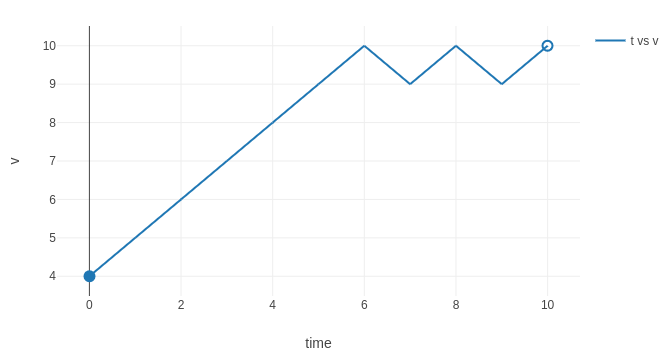
\includegraphics[width=0.75\linewidth]{images/cc_plot.png}
    \caption{Plot of the velocity over time in the cruise control program}
    \label{fig:cc_plot}
\end{figure}

The program starts by assigning the value 4 to variable v. The statement inside the while loop will either accelerate or break, depending on the current velocity, by setting the derivative of $v$, $v'$, to 1 or -1 during 1 second. The while loop indicates that this behavior repeats indefinitely. This appears to be a non-terminating program, because of the infinite while loop, but the evaluation at any specific time will only go through a finite number of iterations of the loop. A plot of the simulated velocity over time can be found in \autoref{fig:cc_plot}.

Despite simple, this example illustrates the basic concepts of a hybrid program, namely the presence of both classical assignment, control structures, etc. as well as differential, continuous constructs and their relation to time.

Among the many difficulties of this paradigm, one of the greatest is the often overlooked matter of precision and error. When developing proper methods of simulation, the standard way to represent numbers is floating point arithmetic, which treats values as a mantissa and an exponent. This system can be, and sometimes is, used to represent numbers with an arbitrary precision, but is usually implemented with a finite precision by limiting the size of the mantissa and exponent. This is enough for most applications, but especially in chaotic systems, where errors compound, the precision limit can be easily exhausted, and any value outputted by the program will stray further and further from the actual value of the calculation. Lince itself uses standard floating point numbers with 64 bits of precision, known as double in most programming languages, which makes it prone to errors when the values get too close to zero. Take the following program as an example:

%   x:=2;
%   x'=1-x for 35;
%   x'=x-1 for 35;
\begin{lstlisting}[caption=Hybrid program showcasing insufficient precision]
x:=1;
x'=-x for 80;
x'= x for 80;
\end{lstlisting}

\begin{figure}
    \centering
    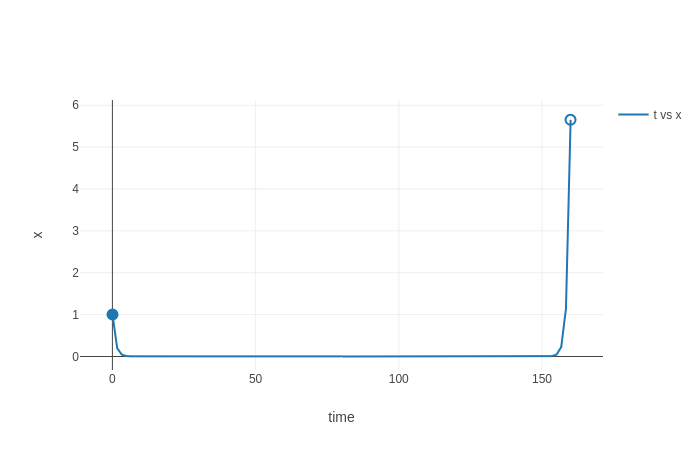
\includegraphics[width=0.75\linewidth]{images/exp_plot.png}
    \caption{Plot of $x$ over time in the exponential program}
    \label{fig:exp-plot}
\end{figure}

\autoref{fig:exp-plot} is a plot of the simulation of variable $x$ over time. Variable $x$ was expected to go from 1 to a very small number at time $t=80$ following a negative exponential ($e^{-t}$), and then follow a positive exponential ($e^t$) afterwards and bounce back to 1 at time $t=160$. But the Lince simulator shows the final value of $x$ as 5.653719, which is clearly an error. This error grows even larger if we replace 80 with even larger values.

Using an arbitrary number of digits to represent values, together with ratio representations (numerator and denominator), allows for the exact representation of all rational numbers, but still leaves open the problem of irrational numbers, which are common when simulating physical systems (when using trigonometric functions, for instance, or with the previous exponential example). Unlike their rational counterparts, it would take an infinite number of digits to represent an irrational number using a regular digit representation. This problem therefore calls for alternative solutions.


\section{Goals}

The goal of the project is the simulation of hybrid systems through the use of exact real arithmetic. More specifically, the project consists of implementing a hybrid system simulator based on preexisting libraries for exact real arithmetic. Simulator performance is expected to be worse than simulators using floating point arithmetic such as the aforementioned tool Lince \cite{goncharov2020}, but should be perfectly faithful to the real system simulated.

The hybrid systems' specification language will be based on a while language with specific constructs to describe the behavior of physical processes. This choice is due to the simplicity and power of the language, which furthermore has a well-established operational semantics that can be used as a basis for implementation. The simulator will be implemented in the Haskell programming language due to its lazy paradigm and use of higher-order functions, which are particularly useful in the context of exact real arithmetic.

\section{Overview}

As a theoretic work, this thesis is mostly about compiling and systematizing already existing research from the fields of exact real arithmetic and hybrid systems. There is a wealth of research on exact real arithmetic, mostly on its more theoretical aspects (a good summary of which can be found in \cite{geuvers07}). This thesis looks at multiple representation strategies from a more practical angle, how they are related, and their unique advantages and disadvantages. As for hybridness, since the topic is already well studied and systematized in the literature, it is presented here in a mostly non-transformative manner, and limited only to the more relevant concepts for the practical implementation of the simulator.

Original theoretical contributions are mostly limited to what was needed to implement the hybrid simulator. Due to fundamental limitations of exact real arithmetic, the simulator can't be implemented directly, instead requiring alternatives and workarounds to combine the two technologies. The main limitation to overcome is the undecidability of comparison in exact real arithmetic, which isn't guaranteed to eventually halt if evaluated totally. The workaround presented in this thesis (\autoref{sec:undecidability}) is instead using partial comparison, up to some accuracy. This workaround forces the operations on hybrid structures to be rewritten as parametrized operations, taking as a parameter the accuracy of the partial comparisons.

The other big challenge to overcome is implementing a differential equation solver that produces a single exact real value as its output. Numerical methods for solving differential equations, like the famous Runge-Kutta\todo{ref}, only generate approximations of the wanted result; and despite being able to reach arbitrarily good approximations (by lowering the step size, for instance), they don't provide strict error bounds for their results, which makes it impossible to convert into an arbitrary-precision real value. The solution presented in this thesis (\autoref{sec:solver}) starts by transforming the equations into a system of polynomial equations. The system is then solved using the equations' Taylor series, obtained with forward automatic differentiation, and a fixed step size to calculate the approximations (which can be arbitrarily improved by taking more and more elements of the Taylor series). The error bound of the results is calculated using the results of the paper "Explicit A-Priori error bounds and Adaptive error control for approximation of nonlinear initial value differential systems" \cite{WARNE20061695}.

On the practical side, this thesis is a comprehensive exposition of the inner workings and functionality of the developed simulator, Jaguar. Beyond the features already discussed, Jaguar supports using all the analyzed exact real arithmetic libraries for its computations (as well as double-precision floating-point numbers as well), and provides an easy base for implementing additional numeric types in the future. Jaguar is also highly configurable, allowing users to choose the parameters of both the simulation and the queries. It also comes with a built-in visualizer using a plotting library, Chart \cite{Chart}.

Though some efforts were made to formalize the new language (see \cref{sec:semantics} for the formalized operational semantics), a lot more could be done in this area, with the ultimate goal being linking the operational and denotational semantics of the language and using the latter to prove its correction.

\section{Document Structure}

After this introduction, \autoref{chap:state_art} gathers the technical background relevant for this project. It first delves into an exploration of existing formalizations and techniques for representing exact real numbers (\autoref{sec:theory}). A study of several open-source libraries follows in \autoref{sec:practice}, where the underlying approaches are compared and critiqued. Then, \autoref{sec:hybrid} lays out the theory behind hybrid systems and presents the underlying challenges of their simulation.

\autoref{chap:implementation} discusses the implementation of the simulator (architecture overview in \autoref{sec:architecture}, followed by the parser in \autoref{sec:parser}, interpreter in \autoref{sec:interpreter}, solver in \autoref{sec:solver} and visualizer in \autoref{sec:visualizer}), and exposes the challenges found along the way and their respective solutions, along with other notable implementation details.

In \autoref{chap:results} the performance of the simulator is discussed, and benchmarking results are presented.

Finally, \autoref{chap:conclusion} talks about the general future direction of this research and lists some next steps towards it.

Throughout this thesis, the reader is assumed to be knowledgeable about partial orders, limits, derivatives, Taylor and Maclaurin series, and monads.\todo{refs}

Functors will be represented with an upper-case sans-serif letter (e.g. $\functor{M}$). If the functor generalizes to a monad, this monad is represented by the same letter in bold font weight. The set of natural numbers is represented with $\N$ and is understood to consist of all non-negative integers ($0 \in \N$). $\R_0^+$ represents the set of non-negative reals. $\overline{\R_0^+}$ denotes the extended non-negative reals (i.e. $\R_0^+$ extended with the infinity value \infty). $[0,\R_0^+)$ is the set of all intervals of the form $[0,d), d \in \R_0^+$ (which includes \emptyset, falling from $d=0$). Finally, $[0,\overline{\R_0^+}\rrparenthesis$ denotes the set of all intervals of form $[0,d], d \in \R_0^+$ or form $[0,d), d \in \overline{\R_0^+}$.


%todo: indice de abreviaturas? so far we got:
% IVP, ODE